
\documentclass[10pt]{report}
\usepackage{amsmath}
\usepackage{latexsym}
\usepackage{amsfonts}
\usepackage[normalem]{ulem}
\usepackage{soul}
\usepackage{array}
\usepackage{amssymb}
\usepackage{extarrows}
\usepackage{graphicx}
\usepackage[backend=biber,
style=numeric,
sorting=none,
isbn=false,
doi=false,
url=false,
]{biblatex}\addbibresource{bibliography-biblatex.bib}

\usepackage{subfig}
\usepackage{wrapfig}
\usepackage{txfonts}
\usepackage{wasysym}
\usepackage{enumitem}
\usepackage{adjustbox}
\usepackage{ragged2e}
\usepackage[svgnames,table]{xcolor}
\usepackage{tikz}
\usepackage{longtable}
\usepackage{changepage}
\usepackage{setspace}
\usepackage{hhline}
\usepackage{multicol}
\usepackage{tabto}
\usepackage{float}
\usepackage{multirow}
\usepackage{makecell}
\usepackage{fancyhdr}
\usepackage[toc,page]{appendix}
\usepackage[hidelinks]{hyperref}
\usetikzlibrary{shapes.symbols,shapes.geometric,shadows,arrows.meta}
\tikzset{>={Latex[width=1.5mm,length=2mm]}}
\usepackage{flowchart}\usepackage[paperheight=11.0in,paperwidth=8.5in,left=1.0in,right=1.0in,top=1.5in,bottom=1.5in,headheight=1in]{geometry}
\usepackage[utf8]{inputenc}
\usepackage[T1]{fontenc}
\TabPositions{0.5in,1.0in,1.5in,2.0in,2.5in,3.0in,3.5in,4.0in,4.5in,5.0in,5.5in,6.0in,}

\urlstyle{same}


 %%%%%%%%%%%%  Set Depths for Sections  %%%%%%%%%%%%%%

% 1) Section
% 1.1) SubSection
% 1.1.1) SubSubSection
% 1.1.1.1) Paragraph
% 1.1.1.1.1) Subparagraph


\setcounter{tocdepth}{5}
\setcounter{secnumdepth}{5}


 %%%%%%%%%%%%  Set Depths for Nested Lists created by \begin{enumerate}  %%%%%%%%%%%%%%


\setlistdepth{9}
\renewlist{enumerate}{enumerate}{9}
		\setlist[enumerate,1]{label=\arabic*)}
		\setlist[enumerate,2]{label=\alph*)}
		\setlist[enumerate,3]{label=(\roman*)}
		\setlist[enumerate,4]{label=(\arabic*)}
		\setlist[enumerate,5]{label=(\Alph*)}
		\setlist[enumerate,6]{label=(\Roman*)}
		\setlist[enumerate,7]{label=\arabic*}
		\setlist[enumerate,8]{label=\alph*}
		\setlist[enumerate,9]{label=\roman*}

\renewlist{itemize}{itemize}{9}
		\setlist[itemize]{label=$\cdot$}
		\setlist[itemize,1]{label=\textbullet}
		\setlist[itemize,2]{label=$\circ$}
		\setlist[itemize,3]{label=$\ast$}
		\setlist[itemize,4]{label=$\dagger$}
		\setlist[itemize,5]{label=$\triangleright$}
		\setlist[itemize,6]{label=$\bigstar$}
		\setlist[itemize,7]{label=$\blacklozenge$}
		\setlist[itemize,8]{label=$\prime$}

\setlength{\topsep}{0pt}\setlength{\parindent}{0pt}

 %%%%%%%%%%%%  This sets linespacing (verticle gap between Lines) Default=1 %%%%%%%%%%%%%%


\renewcommand{\arraystretch}{1.3}

\title{\ \ \ \  Design and Analysis of Algorithms}
\date{}


%%%%%%%%%%%%%%%%%%%% Document code starts here %%%%%%%%%%%%%%%%%%%%



\begin{document}

\maketitle
\par

{\fontsize{15pt}{18.0pt}\selectfont \textbf{\uline{C2 Assignment-2}}\uline{, \textbf{Group-3}}\par}\par


\vspace{\baselineskip}
Pritik Shrivastava – IIT2019192\par

Chetan\ Patidar-\ IIT2019193\ \ \ \ \ \ \ \    \par

Rahul Roy- IIT2019194\par

\ \  \ \ \ \ \ \ \ \ \ \ \ \ \ \ \ \ \ \ \  \tab \ \ \ \ \ \ \ \ \  \tab \ \ \ \ \  \tab \ \ \ \ \  \par


\vspace{\baselineskip}
\begin{multicols}{2}

\vspace{\baselineskip}
{\fontsize{9pt}{10.8pt}\selectfont \textbf{Abstract-Given a gold mine of n$\ast$ m dimensions. Each field in this mine contains a positive integer which is the amount of gold in tons. Initially the miner is at first column but can be at any row. He can move only (right,right up,right down) that is from a given cell, the miner can move to the cell diagonally up towards the right or right or diagonally down towards the right. Find out maximum amount of gold he can collect. }\par}\par


\vspace{\baselineskip}
{\fontsize{9pt}{10.8pt}\selectfont \textbf{\ \ \ \ \ \ \ \ \ \ \ \   \par}\  I. INTRODUCTION}\par


\vspace{\baselineskip}
In simple words, the problem can be explained as follows:\par

The miner starts at the first column, (any row). And after every step he moves one step right into the next column (either towards right or diagonally right), until he reaches the final column.\par

Our job is to make the miner move through the path which gives him the maximum gold and return the maximum amount of gold collected.\par


\vspace{\baselineskip}
We will solve the given problem using dynamic programming approach\par

This report further contains -\par


\vspace{\baselineskip}
II. Algorithm Design\par

III. Algorithm Analysis\par

IV. Experimental Study\par

V. Conclusion\par


\vspace{\baselineskip}

\vspace{\baselineskip}
\ \ \ \ \  \textbf{\ \ \ \ \ \ \  II.A}{\fontsize{9pt}{10.8pt}\selectfont \textbf{LGORITHM DESIGN}\par}\par


\vspace{\baselineskip}
The Algorithm we designed is based on top down approach of dynamic programming to find the most suitable path that provides maximum sum of elements of matrix. The recursive approach calculates the maximum amount of gold that can be obtained from every path in the matrix and stores it in a dp table to reduce time in calculating overlapping sub problems.\par


\vspace{\baselineskip}
\textbf{1.}A dp table of dimension n$\ast$ m is first created and initialized with a value of -1 for all cells.\par


\vspace{\baselineskip}
\textbf{2. }The recursive function gets input in the form of mine matrix and its dimensions(n,m), dp matrix, current row(i) and current column(j).\par


\vspace{\baselineskip}
\textbf{3.}The function calculates the maximum amount of gold that can be obtained if miner starts from the current position(i,j) and stores it in dp table.\par


\vspace{\baselineskip}
\textbf{4}. In every move we find the maximum of right, right\_up, and right\_down and then add it with that mine[i][j] and also store and return the result in dp[i][j].\par


\vspace{\baselineskip}
\textbf{5.} If we have reached outside the dimensions of mine matrix then we return 0. Therefore, when we are in the first row we cannot move right\_up, when we are in last row we cannot move right\_down and when we reach last column the recursive function ends.\par


\vspace{\baselineskip}
\textbf{6.}If we reach any cell from where the maximum amount of gold has already been calculated ie. dp[i][j] is not equal to -1 then we return the value in dp[i][j].\par


\vspace{\baselineskip}
\textbf{7. } We run the following function for every cell in the first column. At last, we find the maximum of all rows and first column and return it as our answer.\par


\vspace{\baselineskip}
\textbf{For example-}\par


\vspace{\baselineskip}
\textbf{Consider input mine matrix as follows:-}\par

mine= $ \{ $ $ \{ $ 10, 20, 1$ \} $ ,\par

\ \ \ \ \ \ \  \tab \  $ \{ $ 30, 10, 100$ \} $ ,\par

\ \ \ \ \ \ \ \  \tab   $ \{ $ 10, 10, 10$ \} $ $ \} $ \par


\vspace{\baselineskip}
We run the recursive function at all the cells in first column and compute our dp table. The cells in last column of mine and dp table are equal. In the second column the dp table is computed as sum of current cell and max of  dp[i+1][j+1],dp[i][[j+1]$\&$ dp[i-1][j+1] (if exists) according to the recursive function.\par

The second column of dp table looks like=$ \{ $ 120,110,110$ \} $ \par

Then the first column of the dp table is filled in a similar manner which gives the dp table as\par

{\fontsize{12pt}{14.4pt}\selectfont dp =\tab \par}$ \{ $ $ \{ $ 130, 120, 1$ \} $ ,\par

\ \ \ \ \ \ \  \tab  $ \{ $ 150, 110, 100$ \} $ ,\par

\ \ \ \ \ \ \ \  \tab  $ \{ $ 130, 110, 10$ \} $ $ \} $ \par


\vspace{\baselineskip}
In the above table, the maximum value in the found in the first column is our required answer ie.\ 150.  \par



%%%%%%%%%%%%%%%%%%%% Figure/Image No: 1 starts here %%%%%%%%%%%%%%%%%%%%

\begin{figure}[H]
	\begin{Center}
		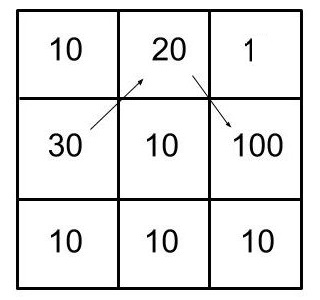
\includegraphics[width=1.94in,height=1.82in]{./media/image1.jpg}
	\end{Center}
\end{figure}


%%%%%%%%%%%%%%%%%%%% Figure/Image No: 1 Ends here %%%%%%%%%%%%%%%%%%%%


\vspace{\baselineskip}
\vspace{\baselineskip}
\textbf{\ \ \ \ \ \ \ \ \  }\par


\vspace{\baselineskip}
\textbf{\ \ \ \ \ \ \ \ \ \ \ \ \  \  \  PSEUDO CODE}\par


\vspace{\baselineskip}

\vspace{\baselineskip}
{\fontsize{12pt}{14.4pt}\selectfont \textbf{ \par}Algorithm} findMaxGold\par

{\fontsize{12pt}{14.4pt}\selectfont  \par}\textbf{Passed} vector<vector<int>> mine\par


\vspace{\baselineskip}
\textbf{function }max\_gold(mine[][],n,m,i,j,dp[][])\par

\textbf{if}(i<0$ \vert $ $ \vert $ i>n-1$ \vert $ $ \vert $ j<0$ \vert $ $ \vert $ j>m-1)\par

\tab return 0;\par

\textbf{end if}\par

\textbf{if}(dp[i][j]!=-1)\par

\tab return dp[i][j]\par

\textbf{end if}\par


\vspace{\baselineskip}
temp1$ \leftarrow $ max\_gold(mine,n,m,i-1,j+1,dp)\par

temp2$ \leftarrow $ max\_gold(mine,n,m,i,j+1,dp)\par

temp3$ \leftarrow $ max\_gold(mine,n,m,i+1,j+1,dp)\par

dp[i][j] $ \leftarrow $  max(temp1,temp2,temp3)\par


\vspace{\baselineskip}
\textbf{return} dp[i][j]\par


\vspace{\baselineskip}
\textbf{function }findmaxgold()\par

n$ \leftarrow $ mine.size()\par

m$ \leftarrow $ mine[0].size()\par


\vspace{\baselineskip}

\vspace{\baselineskip}
for(i=0;i<n;i++)\par

\tab for(j=0;j<m;j++)\par

\tab \tab dp[i][j] $ \leftarrow $ -1\par


\vspace{\baselineskip}
ans$ \leftarrow $ 0\par

for(i=0;i<n;i++)\par

\ \ \ \ \  ans$ \leftarrow $ max(ans, max\_gold(mine,n,m,i,0,dp))\par


\vspace{\baselineskip}
return ans\par


\vspace{\baselineskip}

\vspace{\baselineskip}

\vspace{\baselineskip}

\vspace{\baselineskip}
\textbf{\ \ \ \ \ \ \ \ \ \   III.ALGORITHM ANALYSIS}\par


\vspace{\baselineskip}
\textbf{A. Time complexity}\par


\vspace{\baselineskip}
The\textbf{ }Algorithm uses recursion with memorization to produce a dynamic programming solution. \par

The algorithm on worst case traverses through the whole matrix of n$\ast$ m dimension, hence the worst case time complexity of this algorithm is  \textbf{O(n$\ast$ m)}\par


\vspace{\baselineskip}

\vspace{\baselineskip}
\textbf{B.\ Space\ complexity\    \ \ \ \ \  }\par


\vspace{\baselineskip}
The space complexity of the program is \textbf{O(n$\ast$ m)} as we store the intermediate results in a dp table which has dimensions of n$\ast$ m.\par


\vspace{\baselineskip}
\textbf{\ \ \ \ \ \ \ \  \  IV. EXPERIMENTAL STUDY\  }\par


\vspace{\baselineskip}
\textbf{Graph(Fig .1) }From the graph plotted between the n(no. of rows :x-axis), m(no. of columns :y-axis) and time(z-axis) we can conclude the \textbf{O(n$\ast$ m)} behavior of the algorithm\par


\vspace{\baselineskip}


%%%%%%%%%%%%%%%%%%%% Figure/Image No: 2 starts here %%%%%%%%%%%%%%%%%%%%

\begin{figure}[H]
	\begin{Center}
		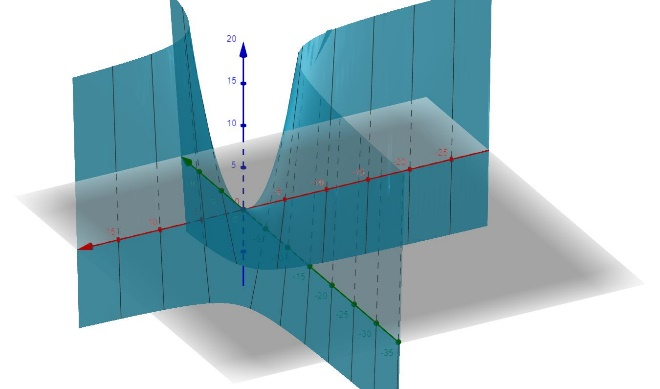
\includegraphics[width=3.0in,height=1.77in]{./media/image2.jpeg}
	\end{Center}
\end{figure}


%%%%%%%%%%%%%%%%%%%% Figure/Image No: 2 Ends here %%%%%%%%%%%%%%%%%%%%


\vspace{\baselineskip}
\vspace{\baselineskip}
{\fontsize{9pt}{10.8pt}\selectfont \ \ \ \ \ \ \ \ \ \ \ \ \ \ \  Fig. 1 .Time complexity curve (N vs t) \par}\par


\vspace{\baselineskip}
\textbf{Graph(Fig .2)} Represents the space complexity \textbf{O(n$\ast$ m)}\par


\vspace{\baselineskip}


%%%%%%%%%%%%%%%%%%%% Figure/Image No: 3 starts here %%%%%%%%%%%%%%%%%%%%

\begin{figure}[H]
	\begin{Center}
		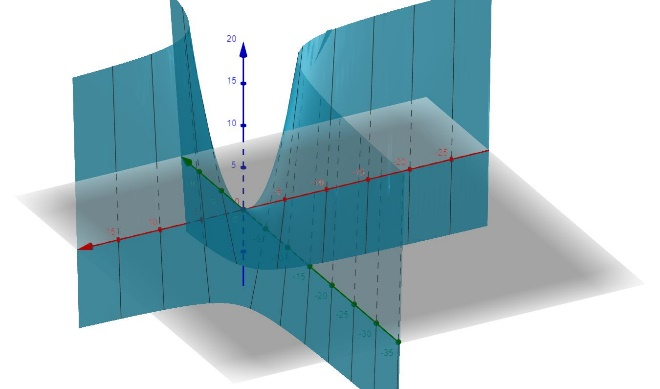
\includegraphics[width=3.0in,height=1.77in]{./media/image2.jpeg}
	\end{Center}
\end{figure}


%%%%%%%%%%%%%%%%%%%% Figure/Image No: 3 Ends here %%%%%%%%%%%%%%%%%%%%


\vspace{\baselineskip}\textbf{\ \ \ \ \ \ \ \ \ \ \ \  }\  {\fontsize{9pt}{10.8pt}\selectfont Fig. 2 .Space\ complexity curve  \par}\par


\vspace{\baselineskip}
{\fontsize{9pt}{10.8pt}\selectfont \ \ \ \ \ \ \ \ \ \ \ \ \ \ \ \  \ \  \par}\textbf{V. CONCLUSION }\par


\vspace{\baselineskip}
In this paper we proposed an algorithm to find the maximum amount of gold a miner can collect by moving only right{\fontsize{9pt}{10.8pt}\selectfont \textbf{(right,right up,right down)\par}} in a mine starting from the first column .The experimental study showed that the time complexity of the algorithm using dynamic programming is \textbf{O(n$\ast$ m) }which depends on the size of the input matrix which is better than the naive approach to use backtracking to produce all the paths that a miner can take from the first column to the last column and for each path calculate the number of gold coins collected on each path which would result in recalculation of recurring subproblems.\par

\textbf{ }\par


\vspace{\baselineskip}
\textbf{\ \ \ \ \ \ \ \ \ \ \  \ \ \ \ \ \ \  }\par

\textbf{\ \  R}{\fontsize{8pt}{9.6pt}\selectfont \textbf{EFERENCES\ \ \  }\par}\par


\vspace{\baselineskip}
{\fontsize{9pt}{10.8pt}\selectfont \ \ \ \ \ [1]  \href{https://www.geeksforgeeks.org}{https://www.geeksforgeeks.org}\par}\par


\vspace{\baselineskip}
{\fontsize{9pt}{10.8pt}\selectfont \ \ \ \  [2]\  Introduction to Algorithms by Thomas H.cormen\par}\par

{\fontsize{9pt}{10.8pt}\selectfont \  \par}\par


\end{multicols}
\printbibliography
\end{document}